\chapter{METODOLOGIA}
\label{cap:desenvolvimento}

Neste capítulo serão apresentados os projetos e tecnologias utilizadas durante o tempo de estágio experienciado.

Na sua grande maioria, os projetos do LEMAF são sistemas web, constituídos de uma aplicação backend e uma frontend.

Durante o desenvolvimento, o backend é, geralmente, compilado no computador do próprio desenvolvedor, porém quando há necessidade de serem feitos testes, é criado um servidor dentro da rede local para que possam ser efetuados os mesmos, sendo mais precisos por conta de estarem em um servidor.

A infraestrutura de servidores do LEMAF são servidores com diversas máquinas, todas rodando NGNIX para prover as aplicações.

O frontend seguia o mesmo processo do backend, porém quando ia para alguma máquina externa, era criado alguma configuração para que o backend servisse o frontend, evitando assim problemas de CORS.

Já o banco de dados era controlado por um DBA (Database Administrator), que criava e gerenciava toda a estrutura de banco, sendo somente necessário aos desenvolvedores discutir melhores soluções e criar demandas para os mesmos realizarem e contemplarem suas necessidades.

Durante o período de estagiário participei de todos squads, trabalhando com diversos times, projetos e tecnologias.

Em minha primeira equipe (Squad 1 - Carreta Furacão), tive como tecnologias necessárias JAVA (backend) e Angular (Frontend) para evoluir os projetos do Cadastro Ambiental Rural, incluindo os projetos SICAR, Central do Responsável Técnico, Central do Proprietário, PRA-OFF.

\begin{figure}[H]
\centering
\caption{SICAR-PA} %legenda
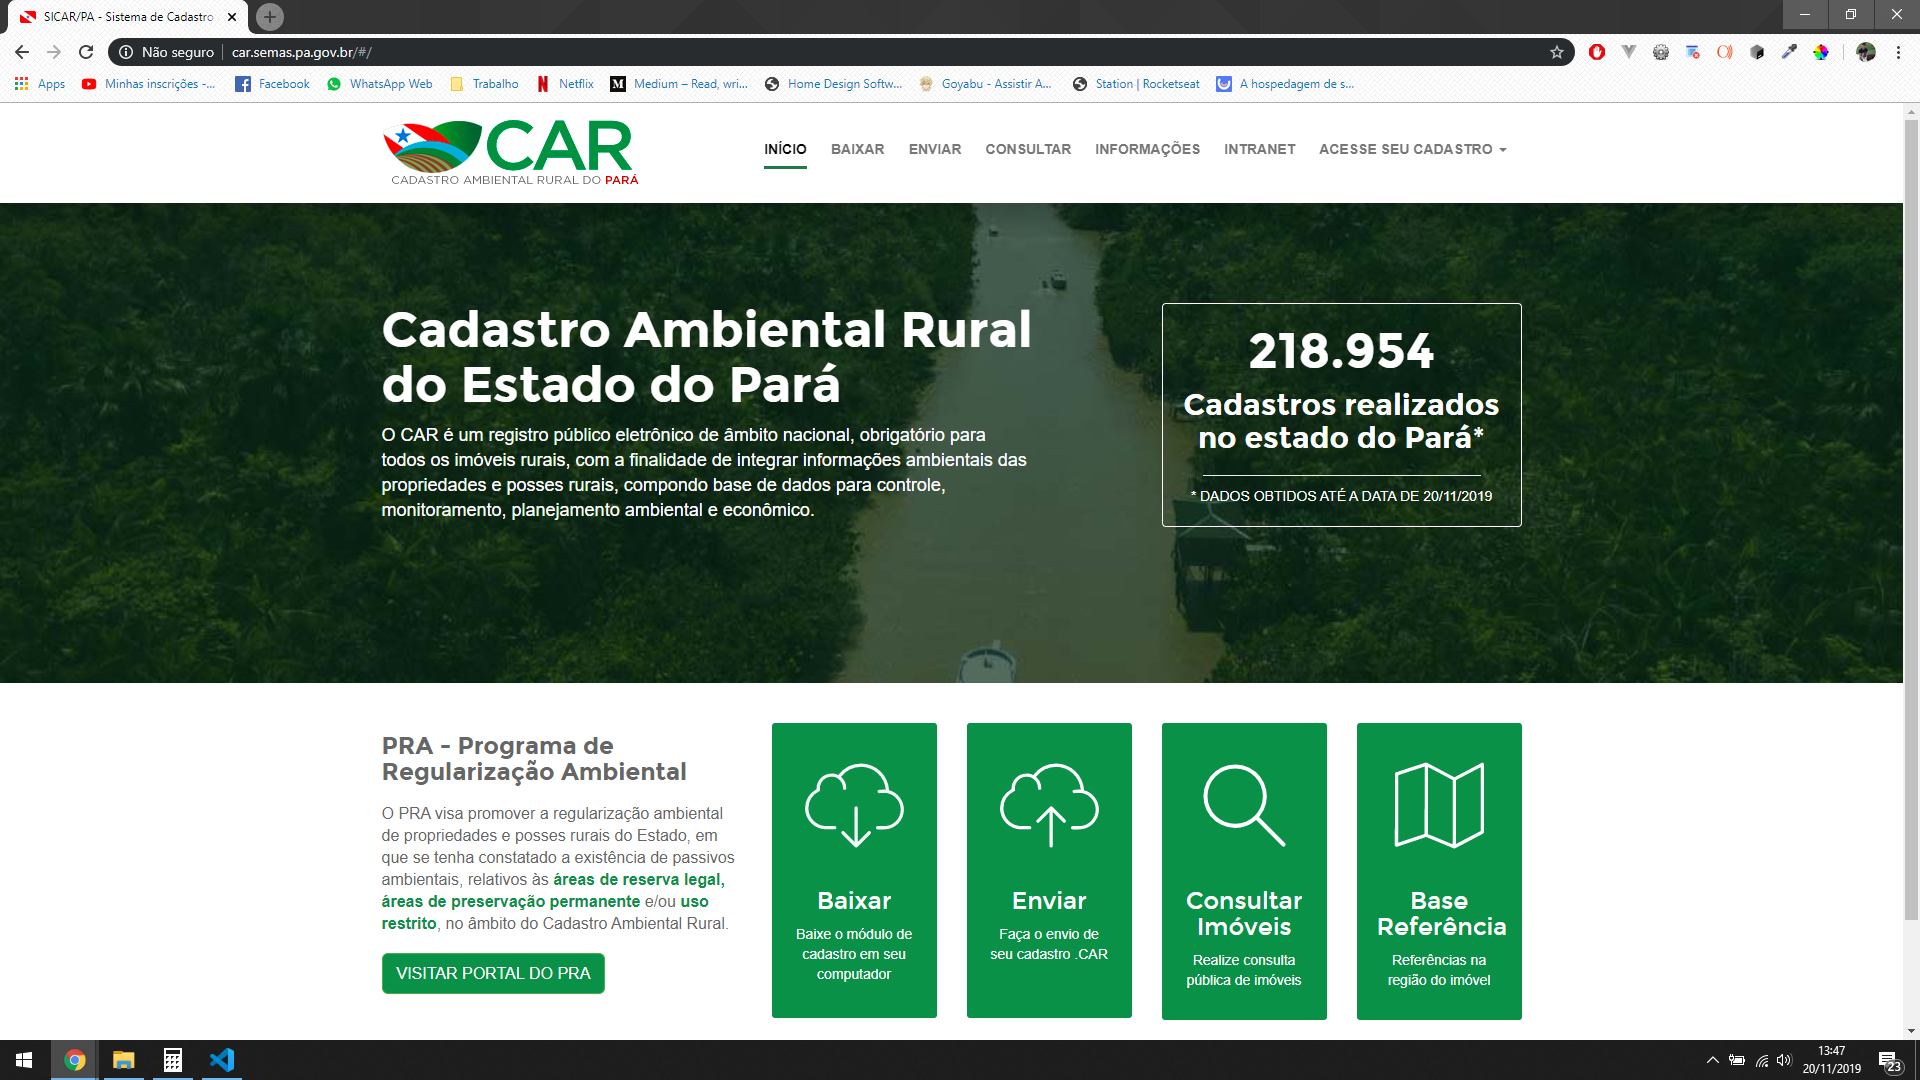
\includegraphics[scale=0.3]{SICAR}\\  % o 0.9 indica 90% do tamanho original
% pdfLaTeX aceita figuras no formato PNG, JPG ou PDF
% figuras vetoriais podem ser exportadas para eps e depois convertidas para pdf usando epstopdf
{\small Fonte: \url{http://car.semas.pa.gov.br/}} %Fonte da imagem
\label{fig:exemplo} %rotulo para refencia
\end{figure}

O projeto do SICAR tinha como objetivo informar e controlar os cadastros ambientais rurais feitos no estado do Pará, sendo necessárias algumas integrações com os módulos do SICAR federal e as Centrais ligadas ao PRA.

\begin{quote}
    Para adequação dos imóveis rurais à nova legislação, foi criado o Cadastramento
Ambiental Rural (CAR) como registro público eletrônico de âmbito nacional,
obrigatório para todos os imóveis rurais, com a finalidade de integrar as informações ambientais das propriedades e posses rurais, compondo base de dados
para controle, monitoramento, planejamento ambiental e econômico e combate
ao desmatamento. - \cite{de2015cadastro}
\end{quote}
\begin{figure}[H]
\centering
\caption{PRA-OFF} %legenda
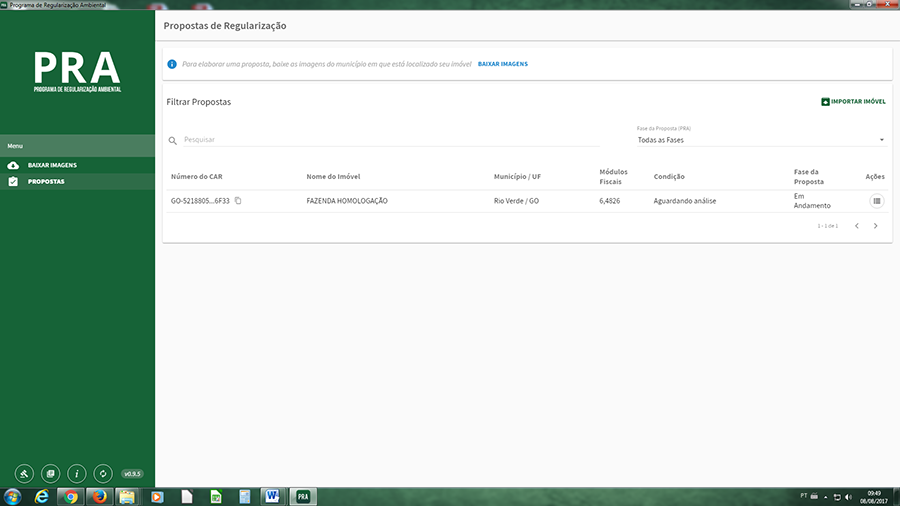
\includegraphics[scale=0.5]{pra-off}\\  % o 0.9 indica 90% do tamanho original
% pdfLaTeX aceita figuras no formato PNG, JPG ou PDF
% figuras vetoriais podem ser exportadas para eps e depois convertidas para pdf usando epstopdf
{\small Fonte: \url{http://www.cprh.pe.gov.br/Controle_Ambiental/Sistema%20Nacional%20de%20Cadastro%20Ambiental%20Rural%20-%20SICAR/PRA/43052%3B53356%3B480802%3B0%3B0.asp}} %Fonte da imagem
\label{fig:exemplo} %rotulo para refencia
\end{figure}

Já o projeto do PRA, não eram possíveis tais integrações, pois ele era um modulo offline, sendo possível a utilização sem internet. Para o desenvolvimento do mesmo, foi necessário estudar sobre electron, uma ferramenta que possibilita criar módulos web em aplicações offline.

Após 5 meses a equipe foi dividida em duas e então foi feita uma redistribuição de projetos, quando fui alocado a tribo Runners. Os projetos principais que contribui durante esse período foram o Consulta Publica - PARÁ e relatórios do PRA.

\begin{quote}
    O objetivo principal é promover as boas
    práticas de manejo florestal, por meio do enriquecimento das florestas secundárias
    remanescentes, localizadas fora das APPs, geralmente compondo a RL. - \cite{de2015cadastro}
\end{quote}
\begin{figure}[H]
\centering
\caption{Consulta publica} %legenda
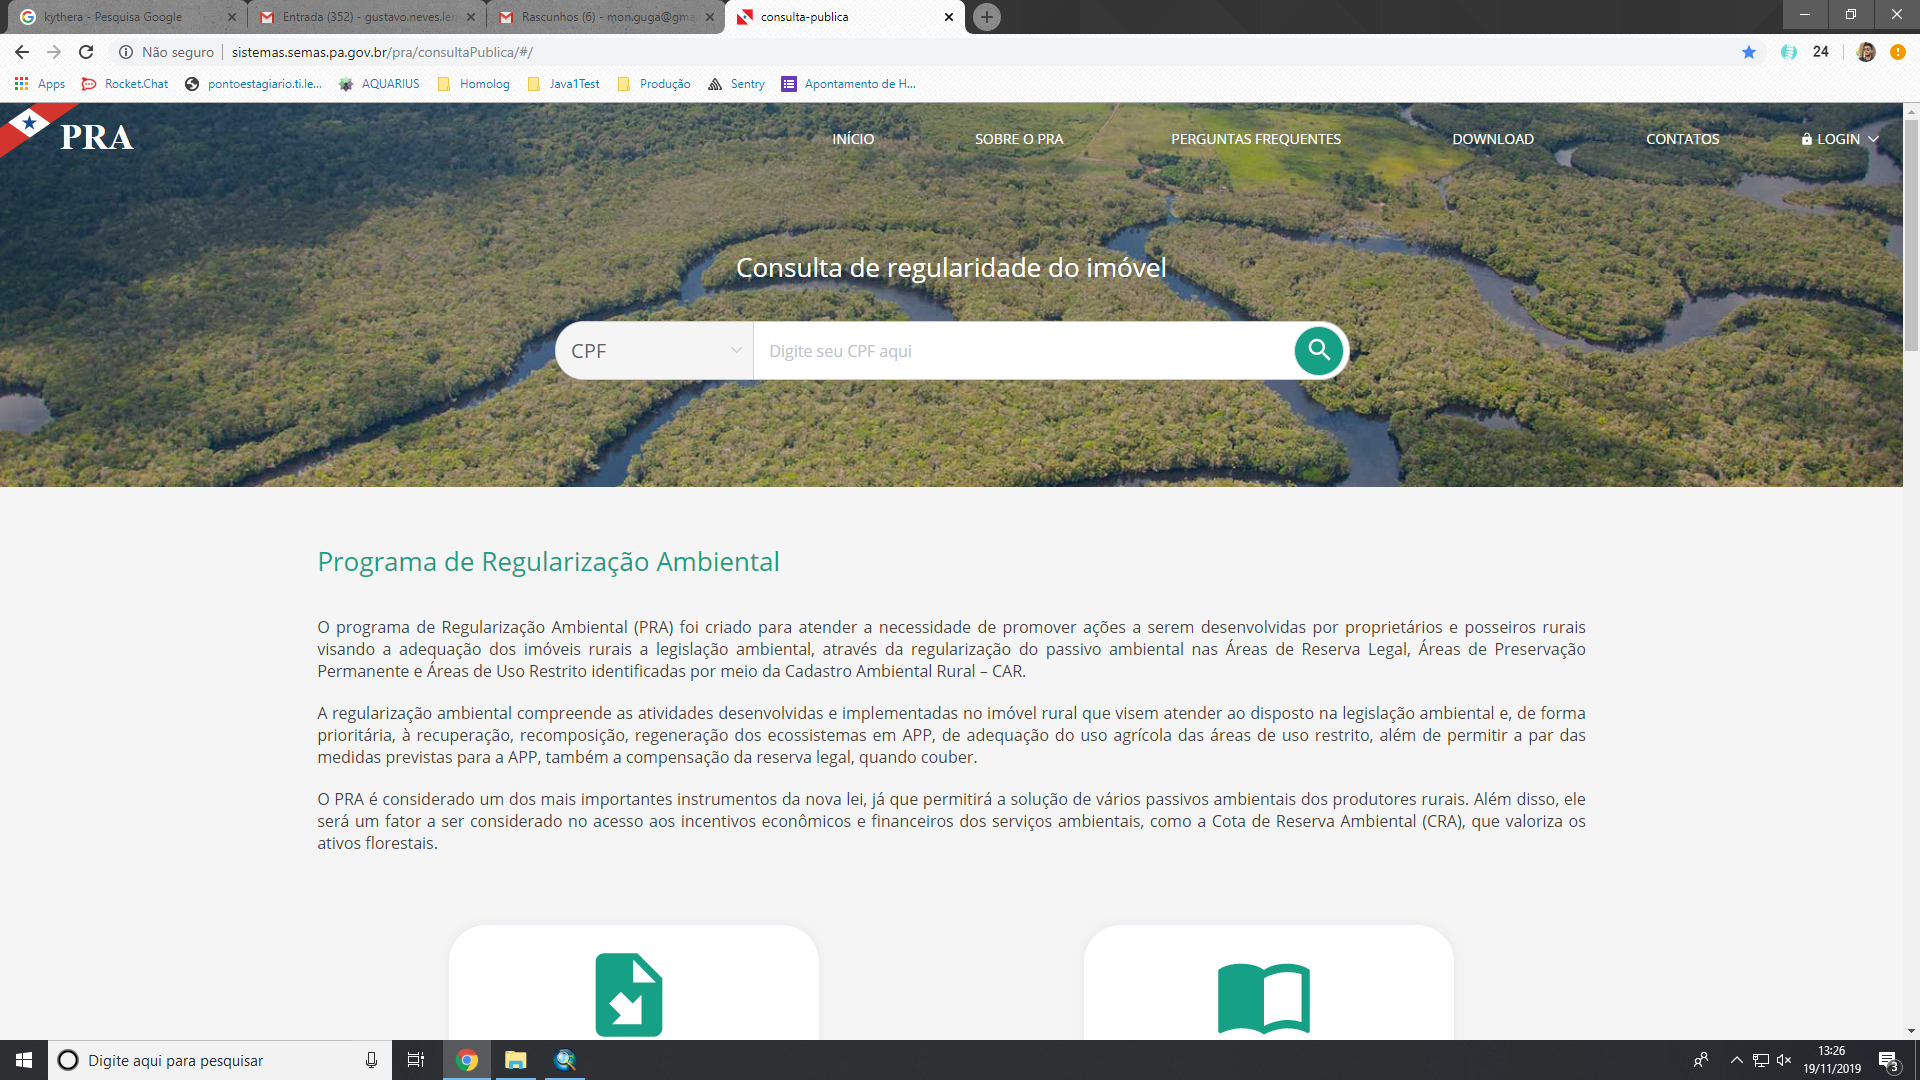
\includegraphics[scale=0.22]{consulta-publica}\\  % o 0.9 indica 90% do tamanho original
% pdfLaTeX aceita figuras no formato PNG, JPG ou PDF
% figuras vetoriais podem ser exportadas para eps e depois convertidas para pdf usando epstopdf
{\small Fonte: \url{http://sistemas.semas.pa.gov.br/pra/consultaPublica/#/}} %Fonte da imagem
\label{fig:exemplo} %rotulo para refencia
\end{figure}

O projeto consulta pública foi o primeiro projeto que tive como objetivo a refatoração, pois se tratava de um projeto legado, utilizava uma das primeiras versões de VueJs no frontend e tinha o layout bem ruim.
Foi a primeira obrigação que tive total responsabilidade, pois tinha que migrar todo o sistema para VueJs 2.0 e refatorar o frontend.

Como era minha primeira experiência com o framework VueJs, foi demandado mais tempo do que o usual, mas tive suporte do meu time que me auxiliava sobre arquitetura, padrões de projetos e boas praticas de programação.
Para melhor aprendizado e controle sobre códigos ruins, todas modificações feitas por mim eram submetidas ao Code Review enviadas para o projeto apenas perante aprovação. 

O projeto consulta pública tinha como objetivo ilustrar aos proprietários de imóveis rurais suas áreas desmatadas, se seus imóveis estavam ou não de acordo com as regularizações ambientais e informações gerais sobre a geometria e hidrografia do terreno.


\begin{figure}[H]
\centering
\caption{Relatórios do PRA} %legenda
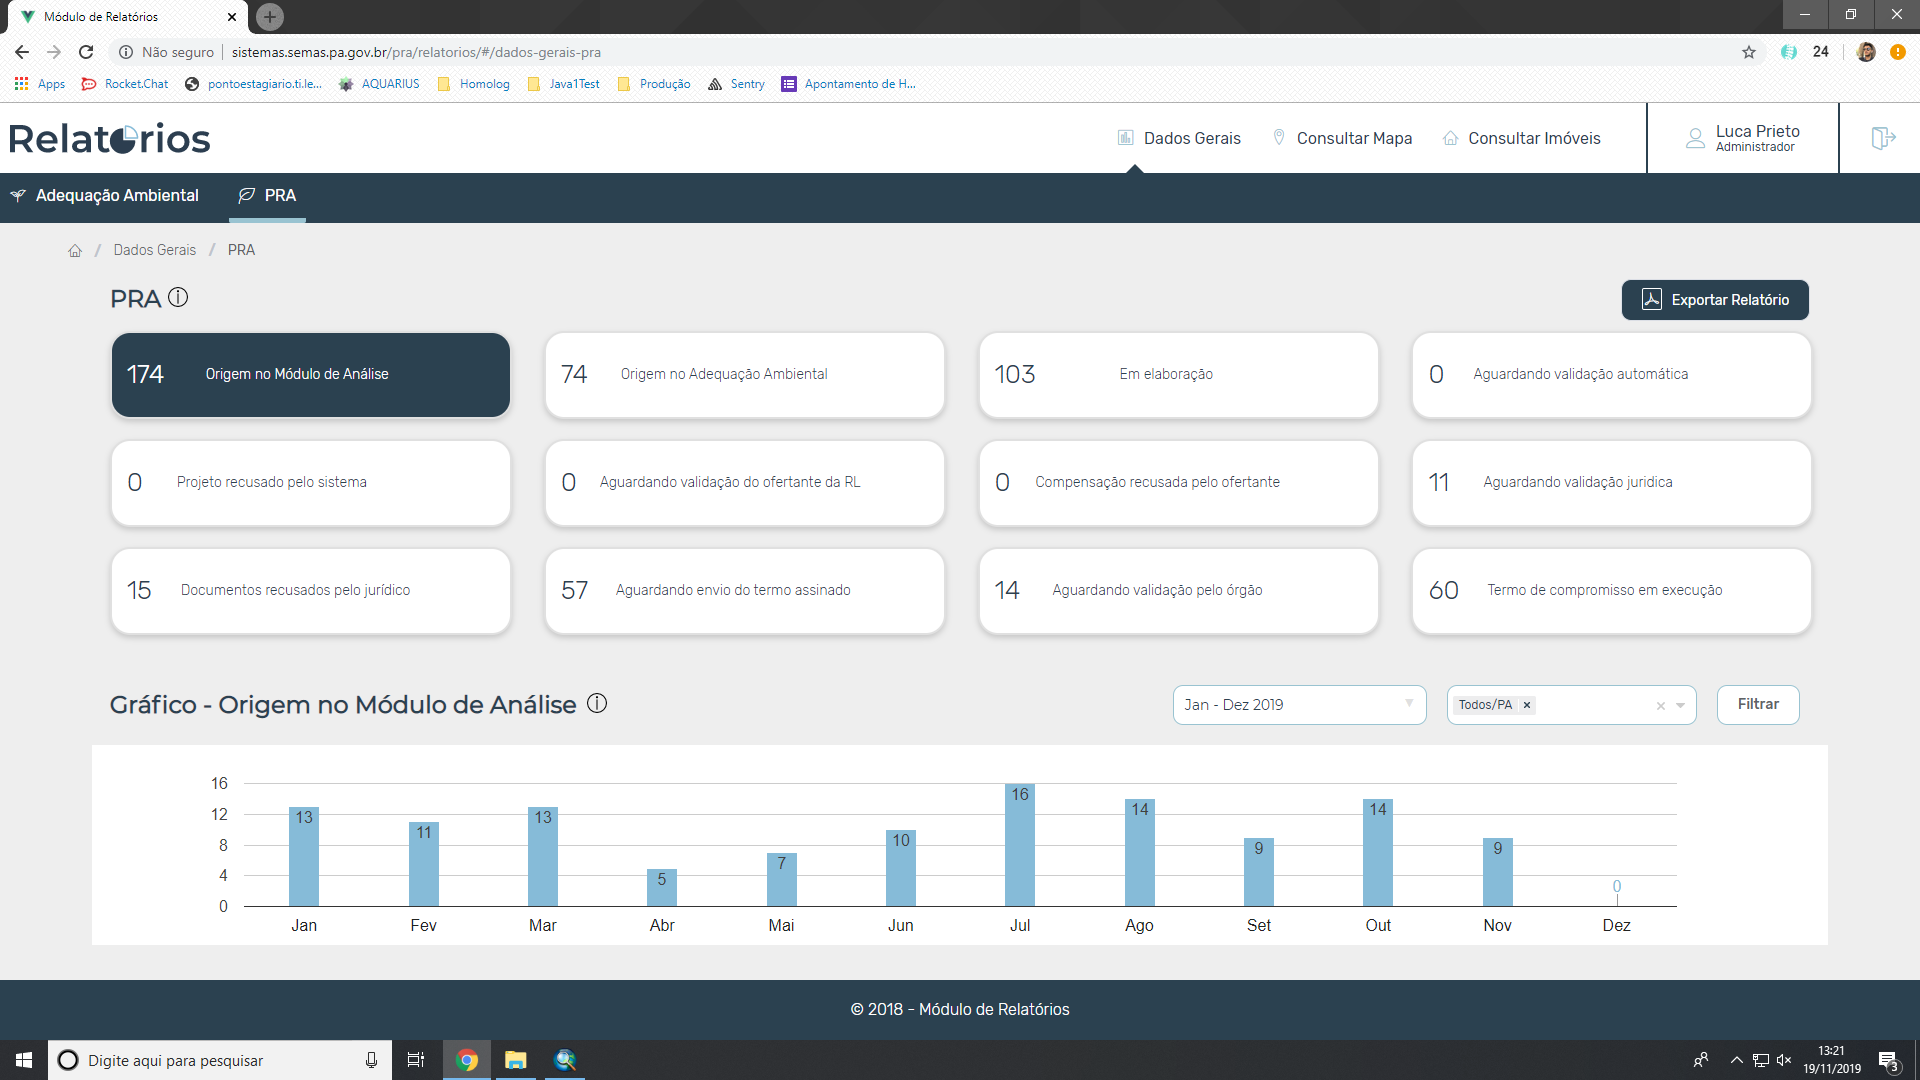
\includegraphics[scale=0.22]{relatorios-pra}\\  % o 0.9 indica 90% do tamanho original
% pdfLaTeX aceita figuras no formato PNG, JPG ou PDF
% figuras vetoriais podem ser exportadas para eps e depois convertidas para pdf usando epstopdf
{\small Fonte: \url{http://sistemas.semas.pa.gov.br/pra/relatorios/#/dados-gerais-adequacao-ambiental}} %Fonte da imagem
\label{fig:exemplo} %rotulo para refencia
\end{figure}

O projeto de relatórios foi o primeiro projeto que tive a honra de iniciar, com uma equipe formada de 4 pessoas (2 desenvolvedores, uma tester e uma PO).
O projeto consistia em uma plataforma de relatórios sobre o Programa de Regularização Ambiental e Adequação Ambiental.

O time teve autonomia de escolha da tecnologia, então pela ótima experiência com VueJs e o alto desempenho de tal, o escolhemos para o frontend.
Porém, pelo baixo conhecimento sobre backend, a escolha da tecnologia foi feita pelo outro desenvolvedor da equipe, que escolheu Spring Boot.
Como minha experiência se limitava apenas a evolução de software, houve diversos gargalos no desenvolvimento, como criação de ambientes, scripts para automatização de deploy entre outros.

Mas após 2 meses, por necessitarem de um desenvolvimento com maior domínio de frontend, fui transferido para uma equipe especial, pois a tal não possuía tribo determinada.
O projeto era uma POC (Prova de conceito) direcionada a uma empresa do ramo de agronomia. Com prazos curtíssimos e complexidade alta, o projeto foi um dos mais difíceis que já trabalhei.
O projeto foi construído utilizando componentização, com o backend feito com uma arquitetura bem definida e documentada para que fosse possível evoluir com o menor nível de dificuldade possível. Devido ao começo bem estruturado e documentado, o projeto foi bem sucedido.

Após esse projeto, fui alocado na tribo Atlântida, onde trabalhei juntamente com mais um desenvolvedor em no projeto SEIRH-CMS.

\begin{figure}[H]
\centering
\caption{SEIRH-CMS} %legenda
\includegraphics[scale=0.22]{SEIRH-CMS}\\  % o 0.9 indica 90% do tamanho original
% pdfLaTeX aceita figuras no formato PNG, JPG ou PDF
% figuras vetoriais podem ser exportadas para eps e depois convertidas para pdf usando epstopdf
{\small Fonte: \url{http://monitoramento.semas.pa.gov.br/SEIRHCMS}} %Fonte da imagem
\label{fig:exemplo} %rotulo para refencia
\end{figure}

O projeto do SEIRH-CMS era um gerenciador de conteúdo da aplicação SEIRH (Sistema Estadual de Informações Sobre Recursos Hídricos do Pará).
A plataforma web do SEIRH já existia, porém não havia comunicação com um backend, então seu conteúdo não era gerenciável. Logo, havia a necessidade de refatoração total do sistema.

\begin{figure}[H]
\centering
\caption{SEIRH} %legenda
\includegraphics[scale=0.22]{SEIRH}\\  % o 0.9 indica 90% do tamanho original
% pdfLaTeX aceita figuras no formato PNG, JPG ou PDF
% figuras vetoriais podem ser exportadas para eps e depois convertidas para pdf usando epstopdf
{\small Fonte: \url{http://monitoramento.semas.pa.gov.br/SEIRH}} %Fonte da imagem
\label{fig:exemplo} %rotulo para refencia
\end{figure}

Então, a refatoração do sistema foi atribuída como tarefa designada ao nosso time.
Como meu conhecimento sobre backend já era mais amplo e devido a tribo Atlântida ser constituída de desenvolvedores DotNet, resolvemos utilizar o framework DotNet Core 2.0, que 
provia diversas funcionalidades e atendia as nossas expectativas e necessidades.
Já o frontend continuou sendo feito com VueJs, uma vez que nossas experiências com tal framework eram recentes.

O prazo para entrega do projeto era curtíssimo de duas sprints (um mês), então optamos por utilizar um quadro kanban para gerenciar as atividades.
Esta foi minha primeira experiência exercendo liderança em estabelecer as prioridades e definir as atividades, definição das atividades e organização no geral.

O projeto foi finalizado com excelência e no prazo estipulado, o que me rendeu nova oportunidade de alocação em um time que já trabalhava com DotNet e necessitava de mais um desenvolvedor.

O projeto desta vez fazia parte de um grande complexo de plataformas que havia sido encomendado por uma empresa de agronomia e tinha muitos componentes de frontend similares entre sí.

Desse fato ocorreu uma iniciativa minha e de outro desenvolvedor de iniciarmos a construção do Design System em um contexto organizacional.
Surgiu então, o Cria Design System\footnote{Disponível em \url{https://criatecnologiainovacao.github.io/cria-design-react/}}, que é uma biblioteca de componentes UI para ReactJs.

Todos os componentes eram criados pelo design do projeto, definindo comportamentos e animações, desenvolvido-os depois. Para a visualização individual dos componentes, utilizamos o StoryBook,
que cria e organiza o catálogo de componentes e então, para compartilhar tal biblioteca para toda a empresa e não surgissem bugs, foram implementados testes automatizados para todos componentes e com necessidade mínima de cobertura de 80\%.

\begin{figure}[H]
\centering
\caption{Cria Design System} %legenda
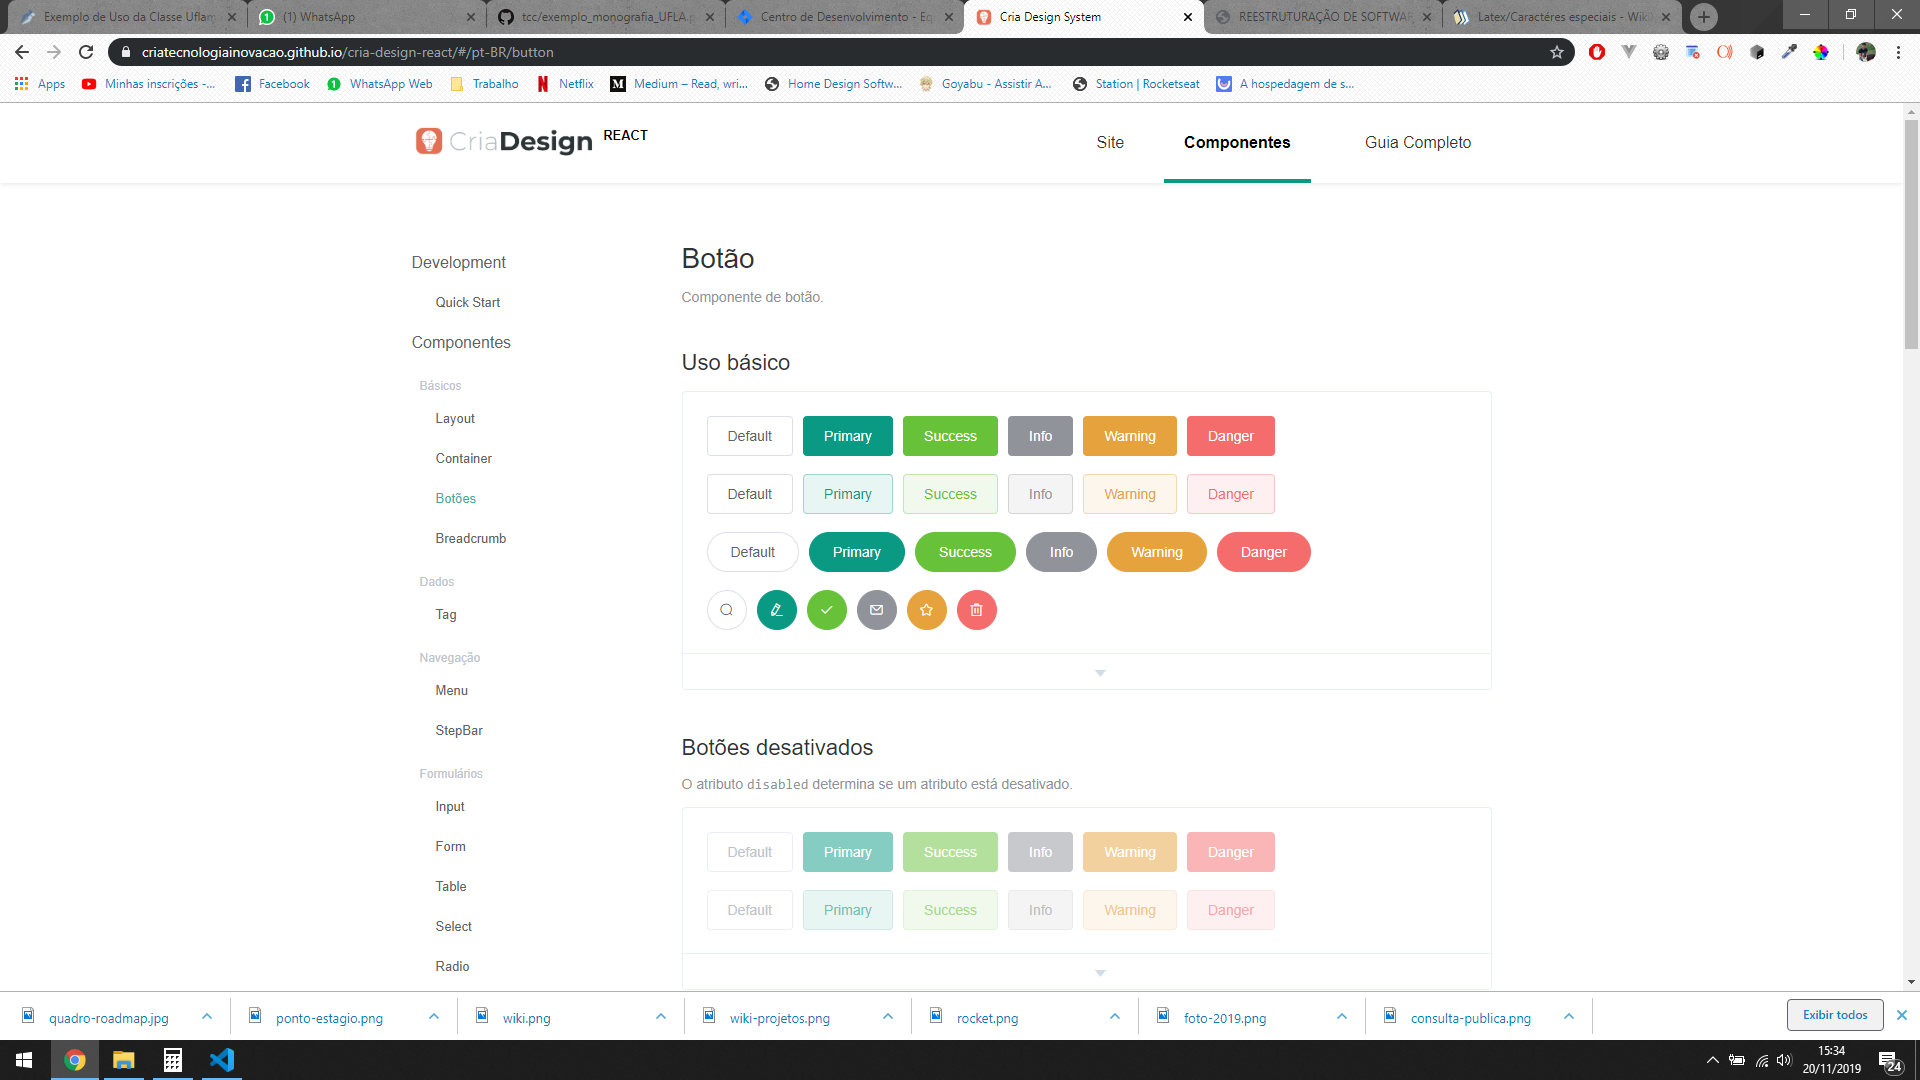
\includegraphics[scale=0.3]{cria-design}\\  % o 0.9 indica 90% do tamanho original
% pdfLaTeX aceita figuras no formato PNG, JPG ou PDF
% figuras vetoriais podem ser exportadas para eps e depois convertidas para pdf usando epstopdf
{\small Fonte: \url{https://criatecnologiainovacao.github.io/cria-design-react/}} %Fonte da imagem
\label{fig:exemplo} %rotulo para refencia
\end{figure}

Após auxiliar com o início do projeto e facilitar o desenvolvimento do mesmo, fui incorporado a uma equipe da mesma tribo, que cuidava de alguns projetos como o SIOUT e SIGER-PA.

\begin{figure}[H]
\centering
\caption{sigerpa} %legenda
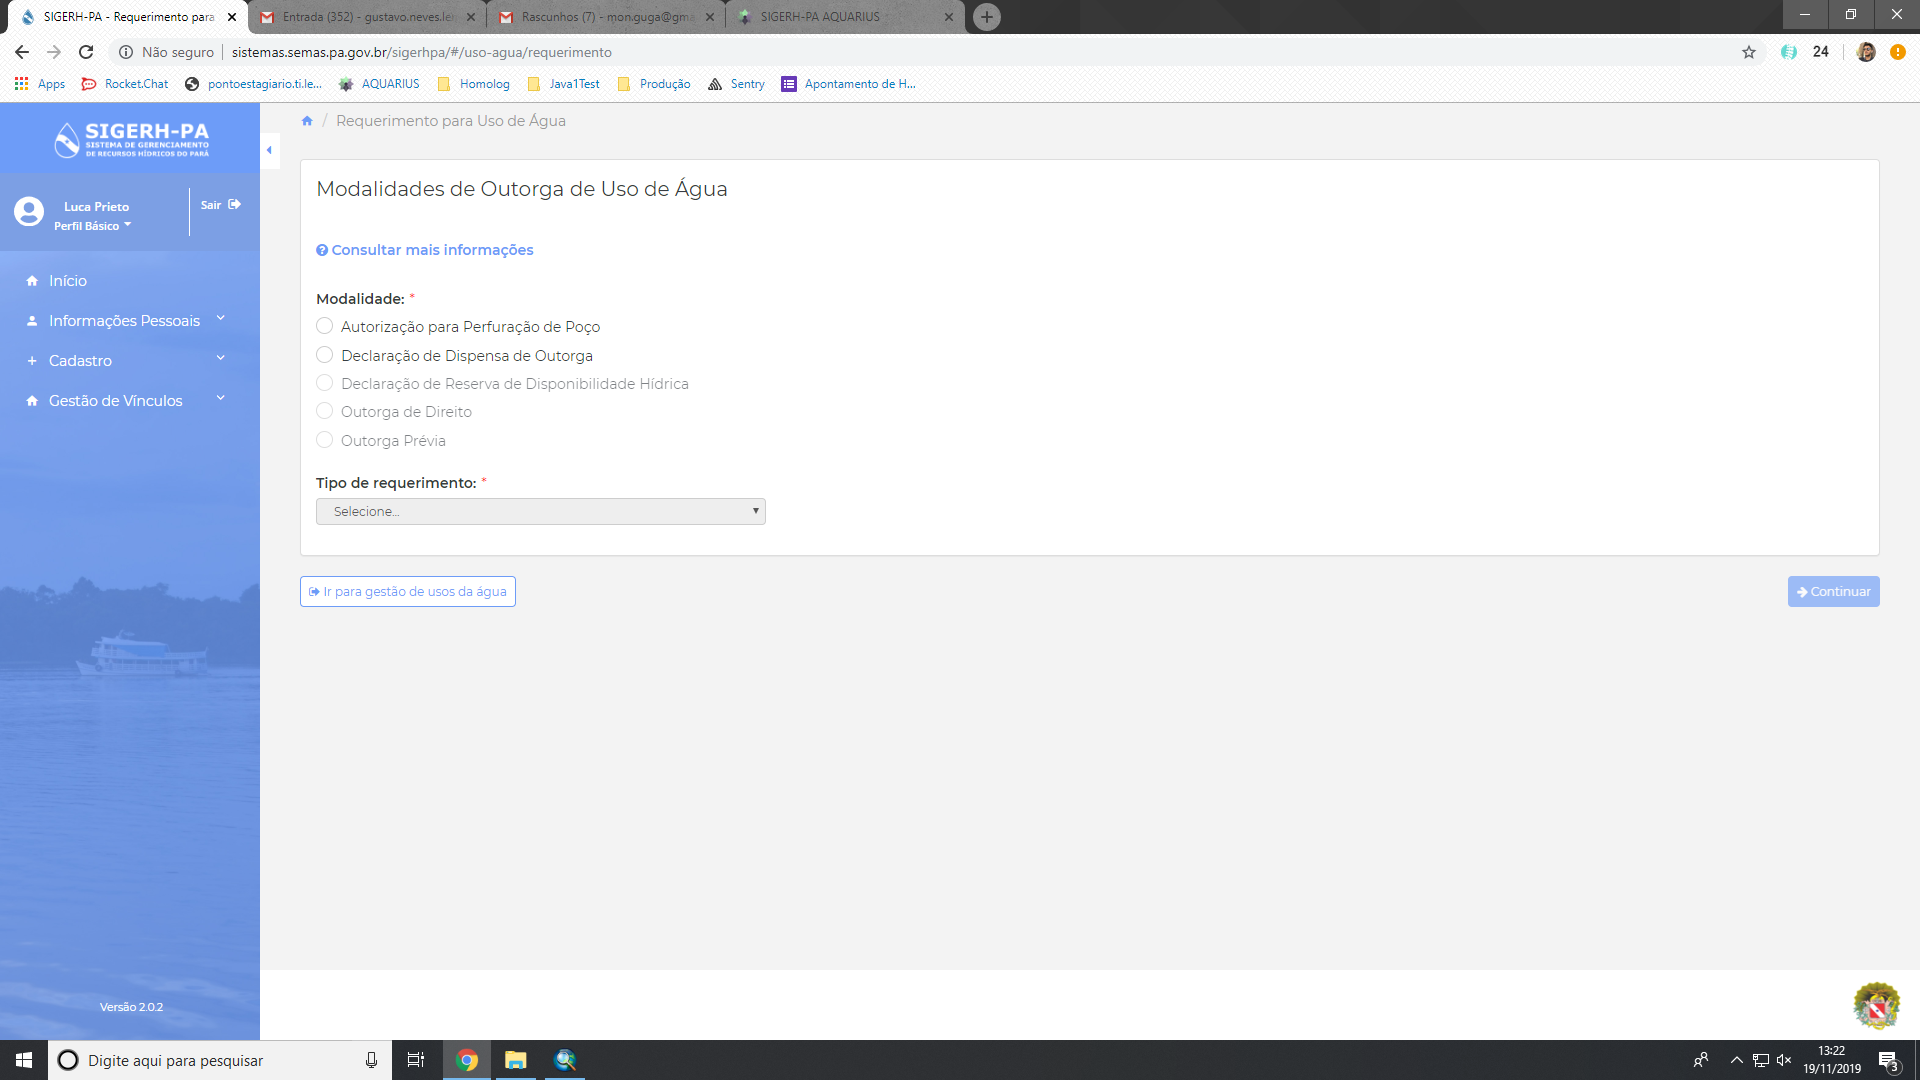
\includegraphics[scale=0.222]{sigerpa}\\  % o 0.9 indica 90% do tamanho original
% pdfLaTeX aceita figuras no formato PNG, JPG ou PDF
% figuras vetoriais podem ser exportadas para eps e depois convertidas para pdf usando epstopdf
{\small Fonte: \url{http://sistemas.semas.pa.gov.br/sigerhpa/}} %Fonte da imagem
\label{fig:exemplo} %rotulo para refencia
\end{figure}

O projeto do SIGER-PA (Sistema de Gerenciamento de Recursos Hídricos do Pará) é uma plataforma de cadastro e regularização de recursos hídricos (poços artesianos, nascentes e outros).
Nele usávamos como backend o framework DotNet Framework 4.0 e como frontend AngularJs.

Ao final do meu estágio, tive como tarefas principais: aprimorar e corrigir tal sistema, que tinha
vários problemas e uma alta complexidade, se tratando de um sistema bastante grande.